\section{Observation and Calculations}

\subsection{Range of $\beta$ particles}

For the measurement of the range of the $\beta$ particles
from Sr-90, first the half thickness is determined for
a source whose range is known (Th-204). Then the half thickness is found out for Sr-90. From that the range and
end point energy of the $\beta$ particles can be found.

During this part of the experiment, the EHT voltage is fixed to 480 V. Distance of source to the detector is 3 cm and distance of absorber to the detector is 2 cm.

Table I shows the background CPS measured for the setup. Table II shows the $\beta$ counts obtained from the detector for both the sources with varying absorber thicknesses.

\begin{table}[]
    \centering
    \begin{tabular}{|c|c|c|}
    \hline
    Background & Average & Avg. Background \\
    Count (in 60s)& Count (in 60s) & CPS (s$^{-1}$) \\ \hline
    54 & \multirow{5}{*}{56} & \multirow{5}{*}{0.933} \\ \cline{1-1}
    53 &  &  \\ \cline{1-1}
    72 &  &  \\ \cline{1-1}
    53 &  &  \\ \cline{1-1}
    48 &  &  \\ \hline
    \end{tabular}
    \caption{Background counts measured for the beta detector}
    \label{tab:1}
\end{table}
\begin{table}[]
    \centering
    \begin{tabular}{|c|c|c|c|c|}
    \hline
    Absorber & Tl-204 & Tl-204 & Sr-90 & Sr-90 \\
    thickness & Count  & CPS & Count  & CPS \\
    (mm) & (in 180s) & (s$^{-1}$) & (in 100s) & (s$^{-1}$) \\ \hline
    0.00 & 6946 & 37.656 & 6191 & 60.977 \\ 
    0.06 & 5336 & 28.711 & 5244 & 51.507 \\ 
    0.12 & 3935 & 20.928 & 4652 & 45.587 \\ 
    0.18 & 3106 & 16.322 & 4231 & 41.377 \\ 
    0.24 & 2419 & 12.506 & 3763 & 36.697 \\ 
    0.30 & 1731 & 8.683 & 3442 & 33.487 \\ 
    0.36 & 1374 & 6.700 & 3282 & 31.887 \\ 
    0.42 & 1002 & 4.633 & 3058 & 29.647 \\ 
    0.48 & 608 & 2.444 & 2799 & 27.057 \\ 
    0.54 &  &  & 2661 & 25.677 \\ 
    0.60 &  &  & 2570 & 24.767 \\ \hline
    \end{tabular}
    \caption{$\beta$ counts observed for both Tl-204 and Sr-90 with varying levels of absorber thickness. The CPS values are corrected based on Table I}
    \label{tab:2}
\end{table}

Fig. \ref{1} and \ref{2} show the plots for $\beta$ CPS vs. surface density of Al, for both the sources respectively. The surface density of Al was calculated as $\rho \times$ thickness, where $\rho = 2.71$ g/cm$^3$ is the volume density. 

\begin{figure}
    \centering
    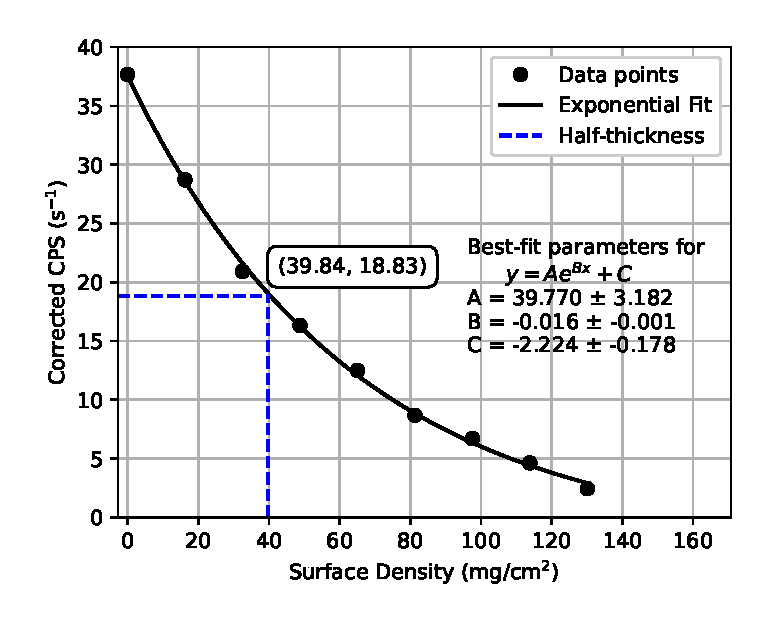
\includegraphics[width=1\columnwidth]{images/Tl.eps}
    \caption{CPS vs. Surface charge density plot for Tl-204}
    \label{1}
\end{figure}

\begin{figure}
    \centering
    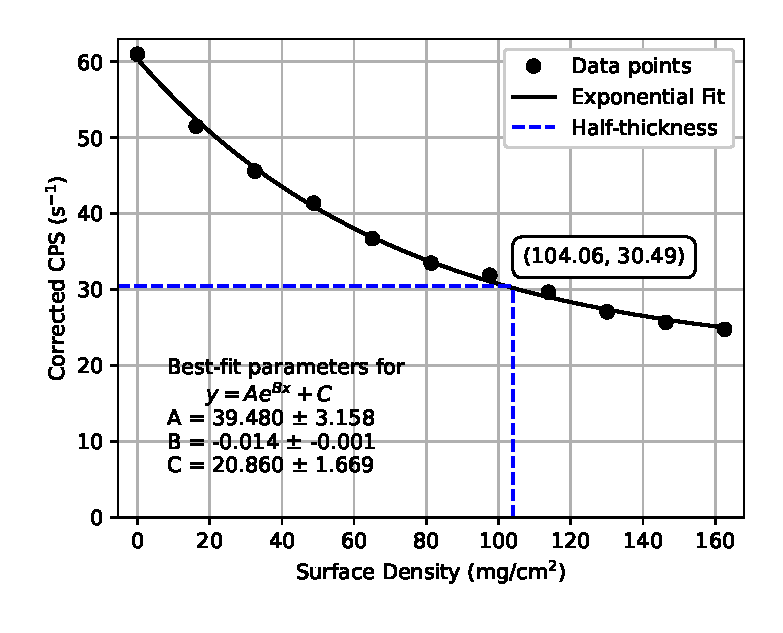
\includegraphics[width=1\columnwidth]{images/Sr.eps}
    \caption{CPS vs. Surface charge density plot for Sr-90}
    \label{2}
\end{figure}

We have fitted an exponential curve to the count vs. surface density data and have observed that the surface density at half the inital CPS is $t_{\frac{1}{2}, \text{Tl}} = 39.84$ mg/cm$^2$ and $t_{\frac{1}{2}, \text{Sr}} = 105.69$ mg/cm$^2$.

Using the known end-point energy of Tl-204 as 0.764 MeV, we can calculate $R_\text{Tl} = 0.307$ g/cm$^2$ using Eq. 1. Now, plugging these in Eq. 2, we get,

\begin{align*}
    R_{\text{Sr}} &= R_{\text{Tl}} \left(\frac{t_{\frac{1}{2},\text{Sr}}}{t_{\frac{1}{2},\text{Tl}}}\right)\\
    &= 0.826 \text{ g/cm}^2
\end{align*}

Pluggin this back into Eq. 1, we get the end-point energy of Sr-90 to be $E_0=1.761$ MeV.

\subsection{Attenuation of Bremsstrahlung}

For measuring the bermsstrahlung effect, the
source and the detector are kept at a fixed distance (6cm)
and then the combinations of absorber plates are put in between them.
Tables III shows the count rates with different combinations of absorbers in different positions.
\begin{table}
	\centering
	\resizebox{\columnwidth}{!}{%
		\begin{tabular}{cccc}
\hline
\multicolumn{4}{|c|}{\textbf{for   Al and perspex}}                                                                                                                   \\ \hline
\multicolumn{1}{|c|}{\textbf{Sl. No.}} & \multicolumn{1}{c|}{\textbf{Absorber}} & \multicolumn{1}{c|}{\textbf{Count}} & \multicolumn{1}{c|}{\textbf{Corrected Count}} \\ \hline
\multicolumn{1}{|c|}{1}                & \multicolumn{1}{c|}{No Absorber}       & \multicolumn{1}{c|}{5662}           & \multicolumn{1}{c|}{5418}                     \\ \hline
\multicolumn{1}{|c|}{2}                & \multicolumn{1}{c|}{Al Facing}         & \multicolumn{1}{c|}{611}            & \multicolumn{1}{c|}{367}                      \\ \hline
\multicolumn{1}{|c|}{3}                & \multicolumn{1}{c|}{Perspex Facing}    & \multicolumn{1}{c|}{571}            & \multicolumn{1}{c|}{327}                      \\ \hline
                                        &                                        &                                     &                                               \\ \hline
\multicolumn{4}{|c|}{\textbf{for Al and copper}}                                                                                                                      \\ \hline
\multicolumn{1}{|c|}{\textbf{Sl. No.}} & \multicolumn{1}{c|}{\textbf{Absorber}} & \multicolumn{1}{c|}{\textbf{Count}} & \multicolumn{1}{c|}{\textbf{Corrected Count}} \\ \hline
\multicolumn{1}{|c|}{1}                & \multicolumn{1}{c|}{No Absorber}       & \multicolumn{1}{c|}{5662}           & \multicolumn{1}{c|}{5418}                     \\ \hline
\multicolumn{1}{|c|}{2}                & \multicolumn{1}{c|}{Al Facing}         & \multicolumn{1}{c|}{373}            & \multicolumn{1}{c|}{129}                      \\ \hline
\multicolumn{1}{|c|}{3}                & \multicolumn{1}{c|}{Copper Facing}     & \multicolumn{1}{c|}{456}            & \multicolumn{1}{c|}{212}                      \\ \hline
                                        &                                        &                                     &                                               \\ \hline
\multicolumn{4}{|c|}{\textbf{for Copper and   Perspex}}                                                                                                               \\ \hline
\multicolumn{1}{|c|}{\textbf{Sl. No.}} & \multicolumn{1}{c|}{\textbf{Absorber}} & \multicolumn{1}{c|}{\textbf{Count}} & \multicolumn{1}{c|}{\textbf{Corrected Count}} \\ \hline
\multicolumn{1}{|c|}{1}                & \multicolumn{1}{c|}{No Absorber}       & \multicolumn{1}{c|}{5662}           & \multicolumn{1}{c|}{5418}                     \\ \hline
\multicolumn{1}{|c|}{3}                & \multicolumn{1}{c|}{Copper Facing}     & \multicolumn{1}{c|}{436}            & \multicolumn{1}{c|}{192}                      \\ \hline
\multicolumn{1}{|c|}{2}                & \multicolumn{1}{c|}{Perspex Facing}    & \multicolumn{1}{c|}{398}            & \multicolumn{1}{c|}{154}                      \\ \hline
		\end{tabular}%
	}
	\caption{Bremsstrahlung data. Each count is for 300s each. The avg. background count was measured to be 244 (from three measurements of 249, 243 and 240).}
	\label{tab:3}
\end{table}

EHT voltage is 480V. The counts are recorded for 180s each.

As we can see, the bremsstrahlung count rate is influenced by the arrangement of absorbent materials. If a metal sheet is positioned closest to the source, a higher count rate is recorded because bremsstrahlung is produced in the aluminum but minimally absorbed by the following Perspex sheet. Conversely, if the $\beta$ rays first pass through a plastic sheet, the resulting bremsstrahlung has lower energy, and a significant portion is absorbed by the subsequent metal sheet. For the Al+Cu combination, we find that the count rate is lower when Al is facing the source. This is because the atomic number of Al ($Z=13$) is lower than that of Cu ($Z=29$). This means there is a higher amount of bremsstrahlung produced in Cu as the $\beta$ particles experience more nuclear force.

\subsection{Backscattering of $\beta$ particles}

To measuring the backscattering radiation, the source and detector are separated by a lead block and they both face the aluminium scatterer, at an angle of 90$^\circ$ with each other. The thickness of the Aluminium scatterer is varied and recorded in Table IV. Fig. \ref{3} shows the count vs. thickness of Al plot.

\begin{table}[]
    \centering
    \begin{tabular}{|c|cc|c|c|}
        \hline
        \multicolumn{1}{|c|}{\multirow{2}{*}{\begin{tabular}[c]{@{}c@{}}Scatterer\\ Thickness \\ (mm)\end{tabular}}} & \multicolumn{2}{c|}{\begin{tabular}[c]{@{}c@{}}Observed\\ Counts\end{tabular}} & \multicolumn{1}{c|}{\multirow{2}{*}{\begin{tabular}[c]{@{}c@{}}Avg.\\ Count\end{tabular}}} & \multirow{2}{*}{\begin{tabular}[c]{@{}c@{}}Net \\ Corrected\\ Count\end{tabular}} \\ \cline{2-3}
\multicolumn{1}{|c|}{} & \multicolumn{1}{c|}{I} & \multicolumn{1}{c|}{II} & \multicolumn{1}{c|}{} &  \\
\multicolumn{1}{|l|}{} & \multicolumn{1}{l|}{} & \multicolumn{1}{l|}{} & \multicolumn{1}{l|}{} & \multicolumn{1}{l|}{} \\ \hline
        0.00 & \multicolumn{1}{c|}{187} & 188 & 187.5 & 0.0 \\ \hline
        0.05 & \multicolumn{1}{c|}{200} & 192 & 196 & 8.5 \\ \hline
        0.10 & \multicolumn{1}{c|}{200} & 189 & 194.5 & 7.0 \\ \hline
        0.15 & \multicolumn{1}{c|}{200} & 224 & 212 & 24.5 \\ \hline
        0.20 & \multicolumn{1}{c|}{214} & 223 & 218.5 & 31.0 \\ \hline
        0.25 & \multicolumn{1}{c|}{229} & 213 & 221 & 33.5 \\ \hline
        0.30 & \multicolumn{1}{c|}{254} & 223 & 238.5 & 51.0 \\ \hline
        0.35 & \multicolumn{1}{c|}{287} & 296 & 291.5 & 104.0 \\ \hline
        0.40 & \multicolumn{1}{c|}{281} & 306 & 293.5 & 106.0 \\ \hline
        0.45 & \multicolumn{1}{c|}{296} & 277 & 286.5 & 99.0 \\ \hline
        \end{tabular}
    \caption{Backscattering data for different scatterer thicknesses. The net corrected count is obtained by assuming the avg. count for 0mm scatterer thickness to be background data.}
    \label{tab:4}
\end{table}

\begin{figure}
    \centering
    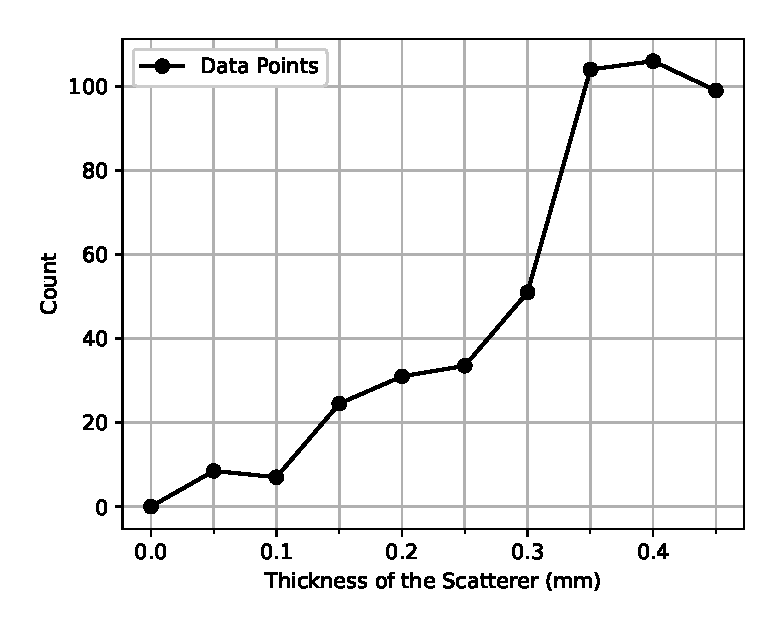
\includegraphics[width=1\columnwidth]{images/backscat.eps}
    \caption{Count vs. Scatterer thickness plot for Sr-204, from backscattering measurements}
    \label{3}
\end{figure}

From Fig. \ref{3}, we can observe that the counts due to back-scattering increases upto a certain thickness of the scatterer and then more or less stabilizes. From this the saturation thickness of the Al can be approximated to be approximately 0.35 mm.

\section{Error Analysis}

For the first part the uncertainity in $R_\text{Sr}$ can be calculated using the error propagation methods on Eq. 2. For that we know that the uncertainity in thickness of the Al is 0.01 mm (least count of the screw gauge), the uncertainity in surface density will be $2.71$ g/cm$^3$ $\times\,0.001$ cm $=2.71\times 10^{-3}$ g/cm$^2$.

\begin{align*}
    \Delta R_{\text{Sr}} &= R_{\text{Sr}} \sqrt{\left(\frac{\Delta t_{\frac{1}{2},\text{Sr}}}{t_{\frac{1}{2},\text{Sr}}}\right)^2 + \left(\frac{\Delta t_{\frac{1}{2},\text{Tl}}}{t_{\frac{1}{2},\text{Tl}}}\right)^2}\\
    &= 0.060 \text{ g/cm}^2
\end{align*}

Similarly, the uncertainity in the end-point energy will be,
\begin{align*}
    \Delta E_{0, \text{Sr}} &= E_{0, \text{Sr}} \left(\frac{\Delta R_{\text{Sr}}}{R_{\text{Sr}}}\right)\\
    &= 0.128 \text{ MeV}
\end{align*}

Since we were only able to vary the thickness of the scatterer in the third part, the uncertainity in the saturation thickness is also the step size we used in the variation, i.e. 0.05 mm.

